\section{Durchführung}

Der Versuchsaufbau ist in Abbildung \ref{fig:aufbau} dargestellt.
\begin{figure}[H]
  \centering
  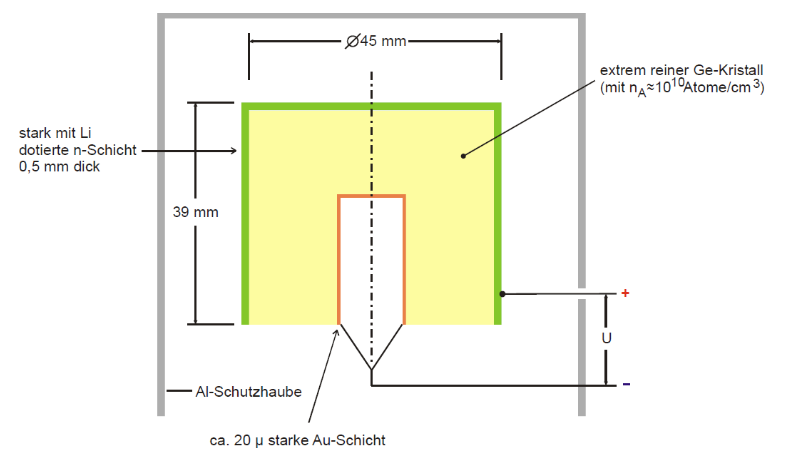
\includegraphics[height=12cm]{Aufbau.png}
  \caption{Versuchsaufbau \cite{skript}.}
  \label{fig:aufbau}
\end{figure}
Zu Beginn des Versuchs wird zunächst der Rezipient evakuiert und anschließend mit Helium
gefüllt. Dann wird das den Rezipienten umgebende Dewargefäß mit flüssigem
Stickstoff gefüllt, um die Probe und den Kupferzylinder auf etwa $\SI{80}{\kelvin}$
zu kühlen, was etwa eine Stunde dauert. \\
Die Temperatur wird über Pt-100-Widerstände mit
digitalen Ohmmetern gemessen, wobei jeweils eines an der
Probe und eines an dem Kupferzylinder angebracht sind.
Der Widerstand von Pt-100-Widerständen ist abhängig von der Temperatur, welche über
die Gleichung
\begin{equation}
   \text{T}= 0,00134\text{R}^2 + 2,296\text{R}-243.02
   \label{eqn:Widerstand}
\end{equation}
berechnet werden kann, wobei der Widerstand hierbei in Ohm und die Temperatur in °C
gegeben sind. \\
Sind die Temperaturen des Kupferzylinders und der Probe in etwa gleich und ausreichend
heruntergekühlt wird der Rezipient erneut evakuiert, um Wärmetransport
durch Konvektion zu vermeiden. Anschließend beginnt der eigentliche
Messvorgang, bei welchem die Probe mit einem Strom von etwa $\SI{170}{\milli\ampere}$
über eine im Inneren angebrachte Heizspule geheitzt wird. Um die zugeführte elektrische
Energie genau bestimmen zu können, wird im Abstand von $\SI{150}{\second}$ jeweils
der Strom und die Spannung notiert, zudem wird auch der Widerstand des Pt-100-Widerstands
notiert. \\
Um den Wärmeübertrag zwischen Kupferzylinder und Probe möglichst gering zu halten,
wird während des Messvorgangs versucht beide auf einer in etwa gleichen Temperatur zu
halten, indem auch der Kupferzylinder mit einer Heizspule geheizt wird, welche
mit etwa $\SI{3}{\ampere}$ bis $\SI{4}{\ampere}$ betrieben wird, wobei der Strom
im Verlauf des Versuchs immer wieder angepasst wird. Auch für den Kupferzylinder
werden alle $\SI{150}{\second}$ Stromstärke, Spannung und Widerstand des
Pt-100-Widerstands notiert. Ist bei der Messung eine Temperatur von etwa
$\SI{170}{\kelvin}$ erreicht werden die Messabstände auf $\SI{300}{\second}$ erhöht.
